\documentclass[../main.tex]{subfile}
\graphicspath{{\subfix{../images}}}
\begin{document}

本节将介绍我们提出的SSD检测框架(\ref{sec:model}节)和相关的训练方法(\ref{sec:training}节)。之后,第3节将介绍了对应数据集的具体模型细节和实验结果。

\subsection{模型} \label{sec:model}

SSD方法基于一个前向传播卷积网络,它产生一个固定大小的边界框集合,并对这些框中存在的物体类别实例进行评分,然后通过一个非最大抑制步骤来产生最终的检测结果。前期的网络层基于用于高质量图像分类的标准结构(在分类层之前截断),我们将其称之基础网络。然后,我们向网络添加辅助结构,以产生具有以下关键特征的检测结果:

\paragraph{用于检测的多尺度特征图}

我们在截断的基础网络的末端添加卷积特征层。这些层的大小逐渐减少,并允许在多个尺度上预测检测。预测检测的卷积模型对于每个特征层都是不同的(参考Overfeat\cite{overfeat}和YOLO\cite{yolo},它们在单一尺度的特征图上进行操作)。

\paragraph{用于检测的卷积预测器}

\begin{figure}[htb]
    \centering
    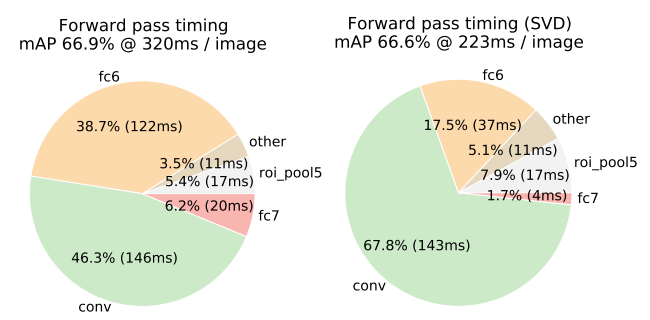
\includegraphics[width=\textwidth]{fig2.png}
    \caption{两个单次检测模型之间的比较:SSD和YOLO\cite{yolo}。我们的SSD模型在基础网络的末端添加了几个特征层,用于预测不同尺度和长宽比的默认框的偏移量及其相关的置信度。具有$ 300 \times 300 $输入大小的SSD在VOC2007\textit{test}中的准确性显着优于其对应的$ 448 \times 448 $YOLO,同时还提高了速度。}
    \label{fig:fig2}
\end{figure}

每个添加的特征层(或来自基础网络的现有特征层)可以使用一组卷积滤波器产生一组固定的检测预测。 这些在图\ref{fig:fig2}中 SSD 网络架构的顶部表示。对于具有$ p $个通道的大小为$ m \times n $的特征层,预测潜在检测参数的基本元素是一个$ 3 \times 3 \times p $小卷积核,它产生类别的分数,或相对于默认框坐标的形状偏移。 在应用卷积核的$ m \times n $位置中的每一个位置,它都会产生一个输出值。 边界框偏移量输出值是相对于每个特征图位置的默认框位置测量的(参见 YOLO\cite{yolo}的架构,该架构在此步骤中使用中间全连接层而不是卷积滤波器)。

\paragraph{默认框和长宽比}

\begin{figure}[htb]
    \centering
    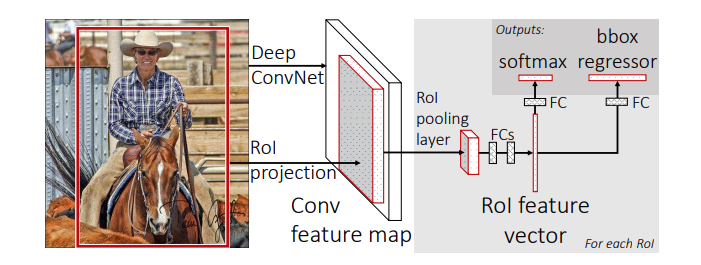
\includegraphics[width=\textwidth]{fig1.png}
    \caption{\textbf{SSD框架。}(a) SSD 在训练期间只需要每个对象的输入图像和ground truth框。 以卷积方式,我们在不同尺寸的几个特征图中(例如(b)和(c)中的$ 8 \times  8 $和$ 4 \times  4$)的每个位置评估一小组(例如 4 个)不同长宽比的默认框。 对于每个默认框,我们预测形状偏移和所有物体类别($\left( c_1, c_2, \ldots, c_p \right)$)的置信度。 在训练时,我们首先将这些默认框与ground truth框匹配。 例如,我们将两个默认框与猫匹配,一个与狗匹配,将它们视为正例,其余视为负例。 模型损失是定位损失(例如 Smooth L1 \cite{fast})和置信度损失(例如 Softmax)的加权和。}
    \label{fig:fig1}
\end{figure}

我们将一组默认边界框与每个特征图单元相关联,用于网络顶部的多个特征图。默认框以卷积方式平铺特征图,这样每个框相对于其对应单元格的位置是固定的。在每个特征图单元格中,我们预测相对于单元格中默认框形状的偏移量,以及每类分数,这些分数表明每个框内是否存在该类的实例。具体来说,对于给定位置的$k$个框中的每个框,我们计算$ c $类分数和相对于原始默认框形状的 4 个偏移量。这导致总共$ (c + 4)k $个卷积核应用于特征图中的每个位置,为$ m \times  n $的特征图产生$ (c + 4)kmn $个输出。有关默认框的说明,请参阅图\ref{fig:fig1}。我们的默认框类似于Faster R-CNN\cite{faster}中使用的锚框,但是我们将它们应用于多个不同分辨率的特征图。在几个特征图中允许不同的默认框形状让我们有效地离散化可能的输出框形状的空间。

\subsection{训练} \label{sec:training}

训练SSD与训练使用区域候选的典型检测器之间的主要区别在于,需要将ground truth信息分配给固定检测器输出集合中的特定输出。YOLO\cite{yolo}中的训练以及 Faster R-CNN\cite{faster}和 MultiBox\cite{multibox1}的区域候选阶段也需要某种版本的分配。一旦确定了此分配,就可以端到端地应用损失函数和反向传播。训练还涉及选择一组默认框和尺度进行检测,以及难负例挖掘和数据增强策略。

\paragraph{匹配策略}

在训练期间,我们需要确定哪些默认框对应于ground truth检测并相应地训练网络。对于每个ground truth框,我们从位置、长宽比和比例不同的默认框中进行选择。我们首先将每个ground truth框与具有最佳jaccard重叠的默认框匹配(如 MultiBox\cite{multibox1})。与MultiBox不同,我们接下来将默认框匹配到任何具有高于阈值 (0.5) 的jaccard重叠的ground truth。这简化了学习问题,允许网络为多个重叠默认框预测高分,而不是要求它只选择重叠最大的一个。

\paragraph{训练目标}

SSD训练目标源自MultiBox目标\cite{multibox1, multibox2},但扩展到处理多个对象类别。让$x_{ij}^p = \left\{ 1, 0 \right\}$是将第$ i $个默认框与类别为$p$的第$j$个ground truth框匹配的指示符。在上面的匹配策略中,我们可以有$\sum_i x_{ij}^p \geq 1$。整体目标损失函数是定位损失(loc)和置信损失(conf)的加权和:
\begin{equation}
    L\left(x, c, l, g\right) = \frac{1}{N}\left( L_{conf}\left(x, c\right) + \alpha L_{loc}\left( x, l, g \right) \right)
\end{equation}
其中$N$是匹配了的默认框数目。如果$N=0$,我们将损失设置为0。定位损失是预测框 ($l$) 和地面实况框 ($g$) 参数之间的Smooth L1损失\cite{fast}。与 Faster R-CNN \cite{faster}类似,我们回归到默认边界框($d$)的中心$\left( xc, cy \right)$及其宽度 ($w$) 和高度 ($h$) 的偏移量。
\begin{equation}
    \begin{aligned}
         & L_{loc}\left( x, l, g \right) & = & \sum_{i\in Pos}^N \sum_{m \in \left\{ cx, cy,w, h \right\} } x_{ij}^k\text{smooth}_{L1}\left( l_i^m - \hat{g}_j^m \right) \\
         & \hat{g}_j^{cx}                & = & \left( g_j^{cx} - d_i^{cx} \right) / d_i^w                                                                                \\
         & \hat{g}_j^{cy}                & = & \left( g_j^{cy} - d_i^{cy} \right) / d_i^h                                                                                \\
         & \hat{g}_j^w                   & = & \log \left( g_j^w / d_i^w \right)                                                                                         \\
         & \hat{g}_j^h                   & = & \log \left( g_j^h / d_i^h \right)
    \end{aligned}
\end{equation}
置信度损失是多类置信度($c$)上的 softmax 损失。
\begin{equation}
    \begin{aligned}
         & L_{conf}\left(x, c\right) & = & -\sum_{i\in Pos}^N x_{ij}^p\log\left(\hat{c}_i^p\right) - \sum_{i\in Neg}\log\left( \hat{c}_i^0 \right) \\
         & \text{where } \hat{c}_i^p & = & \frac{\exp \left( c_i^p \right)}{\sum_p \exp \left(c_i^p\right)}
    \end{aligned}
\end{equation}
并且权重项$\alpha$通过交叉验证设置为1。

\paragraph{为默认框选择尺度和长宽比}

为了处理不同的对象尺度,一些方法\cite{overfeat, spp}建议处理不同的尺寸图像,然后组合结果。然而,通过在单个网络中利用来自多个不同层的特征图进行预测,我们可以模拟相同的效果,同时还可以在所有对象尺度上共享参数。以前的工作\cite{fcn}表明,由于较低层捕获了输入对象的更多细节,所以使用来自较低层的特征图可以提高语义分割质量。类似地,\cite{parsenet}表明添加从特征图中汇集的全局上下文可以帮助平滑分割结果。受这些方法的启发,我们使用底层和高层特征图进行检测。图\ref{fig:fig1}显示了框架中使用的两个示例特征图($8\times 8$ 和 $4\times 4$)。在实践中,我们可以以小计算开销来使用更多的层。

已知来自网络内不同级别的特征图具有不同的(经验上来说)感受野大小 [13]。幸运的是,在SSD框架内,默认框不需要对应每一层的实际感受野。我们设计了默认框的平铺,以便特定的特征图学会对对象的特定尺寸做出响应。假设我们要使用$ m $个特征图进行预测。每个特征图的默认框的尺寸计算如下:
\begin{equation}
    s_k = s_\text{min} + \frac{s_\text{max} - s_\text{min}}{m - 1}\left(k-1\right), k\in\left[1, m\right]
\end{equation}
其中$ s_\text{min} $为 0.2,$s_\text{max}$为 0.9,这意味着最低层的尺度为0.2,最高层的尺度为0.9,并且中间的所有层都是均匀间隔的。我们对默认框施加不同的长宽比,并将它们表示为$a_r \in \left\{ 1, 2, 3, \frac{1}{2}, \frac{1}{3} \right\}$。我们可以计算每个默认框的宽度($w_k^a = s_k \sqrt{a_r}$)和高度($h_k^a = s_k\sqrt{a_r}$)。对于长宽比为1的情况,我们还添加了一个默认框,其尺寸为$s_k^\prime = \sqrt{s_ks_{k+1}}$,从而导致特征图的每个位置有6个默认框。我们将每个默认框的中心设置为$\frac{i+0.5}{\vert f_k \vert}, \frac{j+0.5}{\vert f_k \vert }$,其中$\vert f_k \vert$是第$ k $个正方形特征图的大小, $i, j\in \left[ 0, \vert f_k \vert \right)$。在实践中,还可以设计默认框的分布以最适合特定数据集。如何设计最佳平铺也是一个悬而未决的问题。

通过结合来自多个特征图的所有位置的具有不同尺寸和长宽比的所有默认框的预测,我们有一组多样化的预测,涵盖各种输入对象大小和形状。例如,在图\ref{fig:fig1}中,狗与$ 4\times 4 $特征图中的默认框匹配,但没有与$ 8\times 8 $特征图中的任何默认框匹配。这是因为这些框具有不同的尺度并且与狗框不匹配,因此在训练期间被视为负例。

\paragraph{难负例挖掘}

在匹配步骤之后,大多数默认框都是负例,当可能的默认框数量很大时尤其如此。这引入了正负训练样例之间的显著不平衡。我们没有使用所有的负例,而是使用每个默认框的最高置信度损失对它们进行排序,并选择最高的那些,以便负例和正例之间的比率最多为3:1。我们发现这会导致更快的优化和更稳定的训练。

\paragraph{数据增强}

为了使模型对各种输入对象大小和形状更加鲁棒,每个训练图像都通过以下选项之一随机采样:
\begin{itemize}
    \item 使用全部原始输入图片。
    \item 采样得到补丁,使得与物体的最小jaccard重叠为 0.1、0.3、0.5、0.7 或 0.9。
    \item 随机采样一个补丁。
\end{itemize}
每个采样补丁的大小是原始图像大小的$\left[ 0.1, 1 \right]$,长宽比在$\frac{1}{2}$和$2$之间。如果ground truth框的中心在采样块中,我们保留它的重叠部分。在上述采样步骤之后,除了应用一些类似于[14]中描述的光度失真之外,每个采样的补丁都被重塑为固定大小并以0.5的概率水平翻转。

\end{document}